\documentclass[tikz,border=2pt]{standalone}
\usepackage{amsmath,amssymb}
\usepackage{tikz}
\usetikzlibrary{arrows.meta}

\begin{document}
% Two linear constraints in the plane: independent rows (normals not parallel) meet in a single
% point and cut the dimension by 2; dependent rows describe the same (or parallel) lines and
% remove only one dimension — or nothing feasible at all.
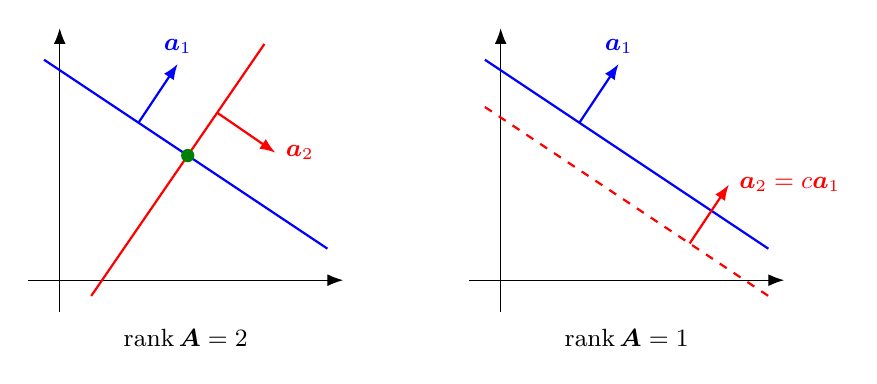
\begin{tikzpicture}[every node/.style={font=\small}, >={Latex[length=2mm]}]
	% Both line endpoints, their intersection and normal arrows use these equations.
    \pgfmathsetmacro{\ms}{-2/3}
    \pgfmathsetmacro{\bs}{8/3}
    \pgfmathsetmacro{\mt}{16/11}
    \pgfmathsetmacro{\bt}{-43/55}
    \pgfmathsetmacro{\ix}{(\bs-\bt)/(\mt-\ms)}
    \pgfmathsetmacro{\iy}{\ms*\ix+\bs}
    \pgfmathsetmacro{\nu}{sqrt(1+\ms*\ms)}
    \pgfmathsetmacro{\nv}{sqrt(1+\mt*\mt)}
    \begin{scope}
        \draw[->] (-0.4,0) -- (3.6,0); \draw[->] (0,-0.4) -- (0,3.2);
        \draw[blue,thick] (-.2,{\ms*(-.2)+\bs}) -- (3.4,{\ms*3.4+\bs});
        \draw[red,thick] (.4,{\mt*.4+\bt}) -- (2.6,{\mt*2.6+\bt});
        \fill[green!50!black] (\ix,\iy) circle (2.4pt);
        \draw[->,blue,thick] (1,{\ms+\bs}) -- ({1-.9*\ms/\nu},{\ms+\bs+.9/\nu}) node[above] {$\boldsymbol{a}_1$};
        \draw[->,red,thick] (2,{2*\mt+\bt}) -- ({2+.9*\mt/\nv},{2*\mt+\bt-.9/\nv}) node[right] {$\boldsymbol{a}_2$};
        \node[anchor=north] at (1.6,-.5) {$\operatorname{rank}\boldsymbol{A}=2$};
    \end{scope}
    \begin{scope}[xshift=5.6cm]
        \draw[->] (-.4,0) -- (3.6,0); \draw[->] (0,-.4) -- (0,3.2);
        \draw[blue,thick] (-.2,{\ms*(-.2)+\bs}) -- (3.4,{\ms*3.4+\bs});
        \draw[red,thick,dashed] (-.2,{\ms*(-.2)+\bs-.6}) -- (3.4,{\ms*3.4+\bs-.6});
        \draw[->,blue,thick] (1,{\ms+\bs}) -- ({1-.9*\ms/\nu},{\ms+\bs+.9/\nu}) node[above] {$\boldsymbol{a}_1$};
        \draw[->,red,thick] (2.4,{2.4*\ms+\bs-.6}) -- ({2.4-.9*\ms/\nu},{2.4*\ms+\bs-.6+.9/\nu}) node[right] {$\boldsymbol{a}_2=c\boldsymbol{a}_1$};
        \node[anchor=north] at (1.6,-.5) {$\operatorname{rank}\boldsymbol{A}=1$};
    \end{scope}
\end{tikzpicture}
\end{document}
